\section{Fixing the POSIX File Interface}
\label{sec:noposix}

Both \DAChell{} and \CChell{} transparently provide a POSIX-compatible
interface, so no changes to the application are needed.  This means, however, that applications must use POSIX-style file access functions and some of these are a poor match for NVMM.
In particular, the POSIX interface
requires the programmer to specify the buffer that \texttt{read()} copies data to.
POSIX places no constraints on the size
or alignment of the buffer, so a copy operation is usually unavoidable.  For
slow disks and even SSDs, the cost of this copy is small.

%\cfigure[Graphs/latency-break-quill.pdf,{\figtitle{Chell-Direct 4~kB read/write latency breakdown. Memory copy accounts for 76\% of total latency. Page table is populated on file open, so the page fault overhead is eliminated.}},fig:latency-break]

But for \DAChell{} and \CChell{}, the relative cost is much larger.
Figure~\ref{fig:latency-break} shows the latency breakdown of 4~kB read and
write operations of \DAChell{} with page table populated and page fault overhead
eliminated.  The memory copy accounts for 76\% for 4~kB
read and 77\% for 4~kB write. For \CChell{}, the situation is similar.
This high overhead of memory copying makes the POSIX interface
itself a major impediment to exploiting the performance of NVMM.

To eliminate it, we propose a new file read interface optimized for
NVMM-based storage systems.  The interface provides a new function:

\vspace{1em}
\begin{tabular}{l}
ssize\_t \grb{}(int fd, char **buf, size\_t count);\\
%ssize\_t \gwb{}(int fd, char **buf, size\_t count);\\
\end{tabular}
\vspace{1em}

\ignore{How do writes work in this interface?  There's something missing here:  \gwb{} doesn't actually have any input data, right?  This gets me the address, but then I have to copy the data there, I guess.  That means I need to ensure that that memory won't go anywhere while I'm writing, and I need to make some other call to make sure that durability is ensured.  I think the best bet would be to just worry about reads, especially given the time remaining.}
\ignore{Yes. write is much more complicated.}

The interface is similar to the conventional \texttt{read}, except that calls
to \texttt{\grb{}} return a buffer to programmer via the \texttt{buf}
parameter.  The \texttt{*buf} contains a portion of the target file
(\texttt{fd}), starting from current file offset and extending for up to
\texttt{count} bytes.  The return value is the actual length of the memory
region.  No copying is necessary.  We added the \grb{} interfaces based to
\DAChell{}.

\ignore{
\begin{figure}[htb]
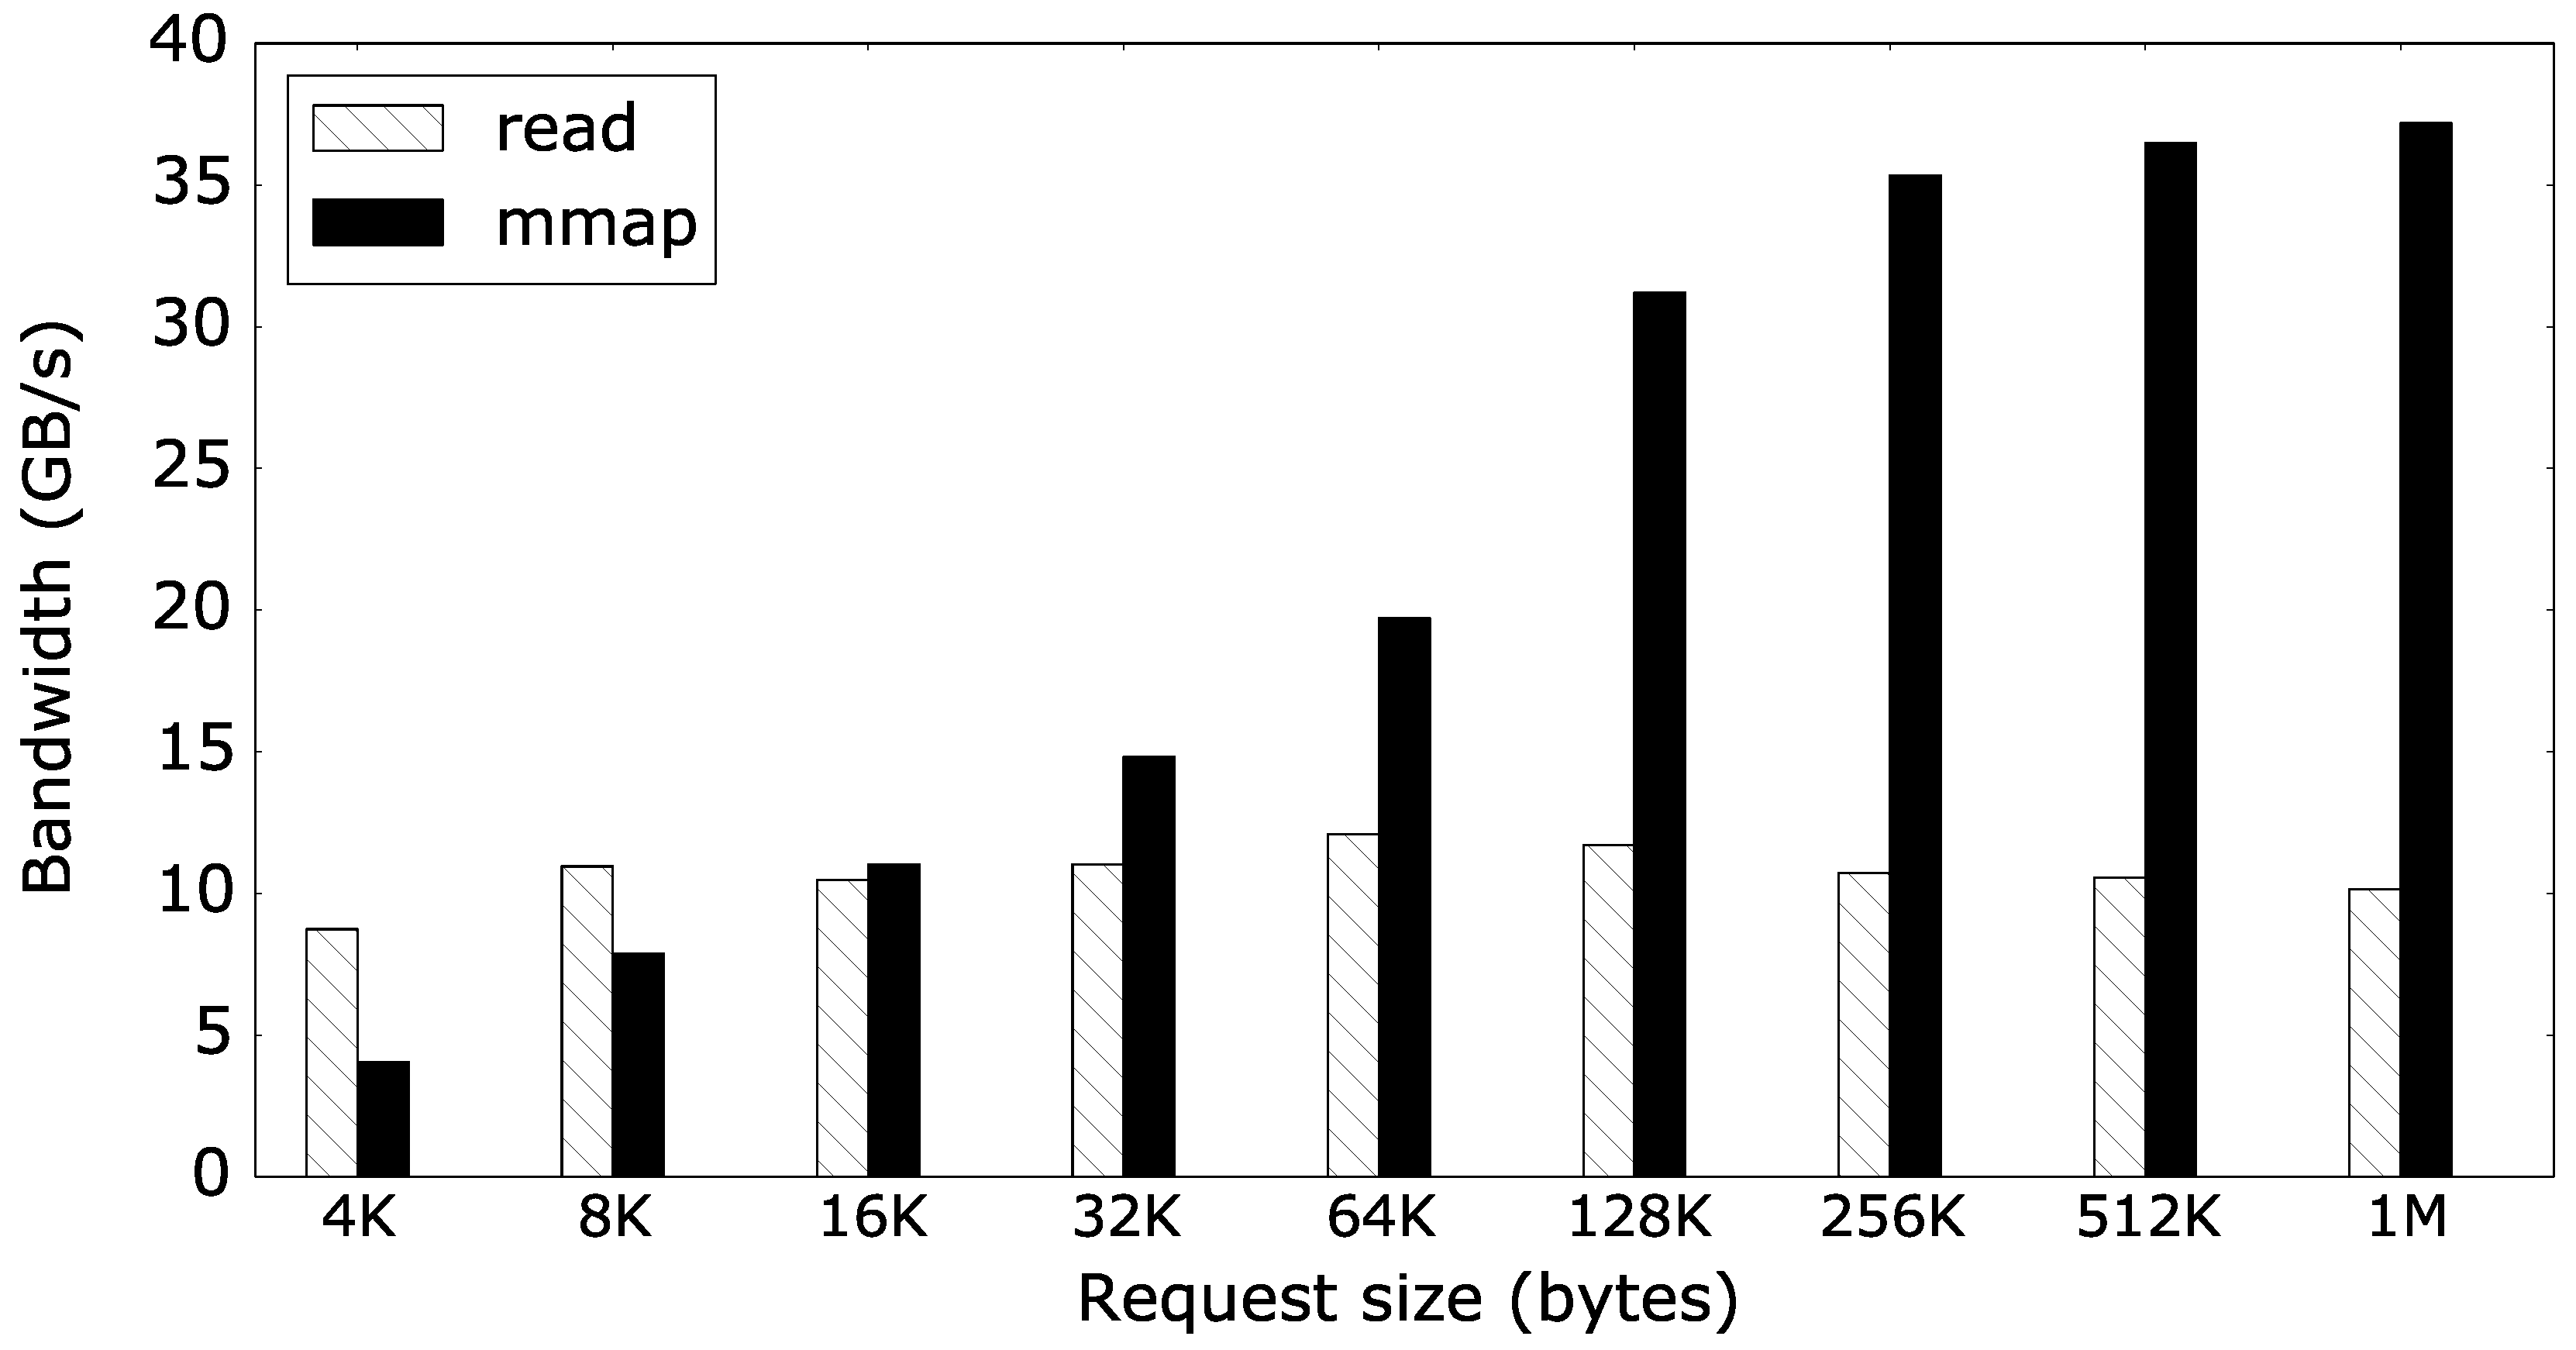
\includegraphics[width=\linewidth]{Graphs/mmap.pdf}
\caption{mmap performance}
\label{fig:mmap}
\end{figure}
}

\cfigure[Graphs/noposix.pdf,{\figtitle{\grb{} interface latency for different request sizes: latency of PMFS and \DAChell{} increases with request size, while \grb{} has constant latency}},fig:noposix]

\ignore{
Figure~\ref{fig:mmap} compares the performance of \grb{} and \texttt{read}
for files stored in NVMM with PMFS.  Conventional \andiry{\texttt{read} is faster for request sizes
below 8~kB WHy is this?}, but \grb{} outperforms \texttt{read} by up to 366\%. This is
because \grb{} calls \texttt{mmap()} for each request\andiry{why?}, for small
request the overhead of mmap operation (about 1000~ns) is larger than the
\texttt{memcpy} operation performed by \texttt{read} (about 400~ns for 4~kB) , but
for larger requests, the overhead of \grb{} is a
page fault to setup the persistent memory page in the page table
(about 100~ns), which is much smaller than a 4~kB \texttt{memcpy} of POSIX
read. \andiry{This seems like a pretty inefficient way to do this.  If the file is already in memory, for \DAChell{}, the latency for \grb{} should be just the lookup time in the btree}
}

Figure~\ref{fig:noposix} compares the performance of the normal POSIX interface
and \texttt{\grb{}} for a sequential read workload running on PMFS with
\Chell{} enabled.  The copy that the POSIX interface requires causes latency to
increase linearly with request size.  \texttt{\grb{}} does not do any copying, so
latency is nearly constant.  For 4~kB request, \grb{} outperforms POSIX for
4.2\x{}, and for 1~MB request, \texttt{\grb{}} achieves performance gain up to
700\x{}.


